%/*% pdflatex -file-line-error -interaction nonstopmode %

\documentclass{article}
\usepackage{graphicx}
\usepackage{amsmath}
\usepackage{amsfonts}
\usepackage{bookmark}
\usepackage{booktabs}
\usepackage{exercises}
\graphicspath{ {./images/test} }
\usepackage{indentfirst}
\usepackage{amsthm}
\usepackage{yhmath}
\usepackage{placeins}
\newcommand*{\oldneg}{\mathord{\sim}}
\newcommand\showdiv[1]{\overline{\smash{)}#1}}
\newcommand\Mydiv[1]{%
\smash{\raise.3ex\hbox{$\big)$}}\mkern-8mu
        \overline{\enspace\strut#1}}
\setlength{\tabcolsep}{5pt}
\theoremstyle{definition}
\newtheorem{definition}{Definition}

\setlength{\parindent}{.5in}
\setlength{\parskip}{12pt}
\renewcommand{\arraystretch}{2}

\title{Test (Page 159)}
\begin{document}
\maketitle

\section*{1}
\[ x^3\times x^2\times x^{-4}=x^{3+2-4}=x^1=x \]
Product of Powers Property.

\section*{2}
\[ (2x^{-2}y^3)^{-5}=2x^{-2\times -5}y^{3\times -5}=2x^{10}y^{-15}=2x^{10}\frac{1}{y^{15}} \]
Power of a Product Property, Power of a Power Property, Negative Power Property.

\section*{3}
\[ (\frac{x^{-4}}{y^2})^{-2}=\frac{x^{-4\times -2}}{y^{2\times -2}}=\frac{x^8}{y^{-4}}=x^8y^4 \]
Power of a Quotient Property, Power of a Power Property, Negative Power Proeprty.

\section*{4}
\[ \frac{3(xy)^3}{27x-5y^3}=\frac{3x^3y^3}{27x-5y^3} \]
Power of a Product Property.

\section*{5}
Because this is a polynomial of odd degree (3) such that the leading coefficient is negative, $f(x)\rightarrow +\infty$ as $x\rightarrow -\infty$ 
and $f(x)\rightarrow -\infty$ as $x\rightarrow +\infty$. Also, by the rational roots theorem, we can tell that the only rationl zero of $f(x)$ 
is at $x=0$:
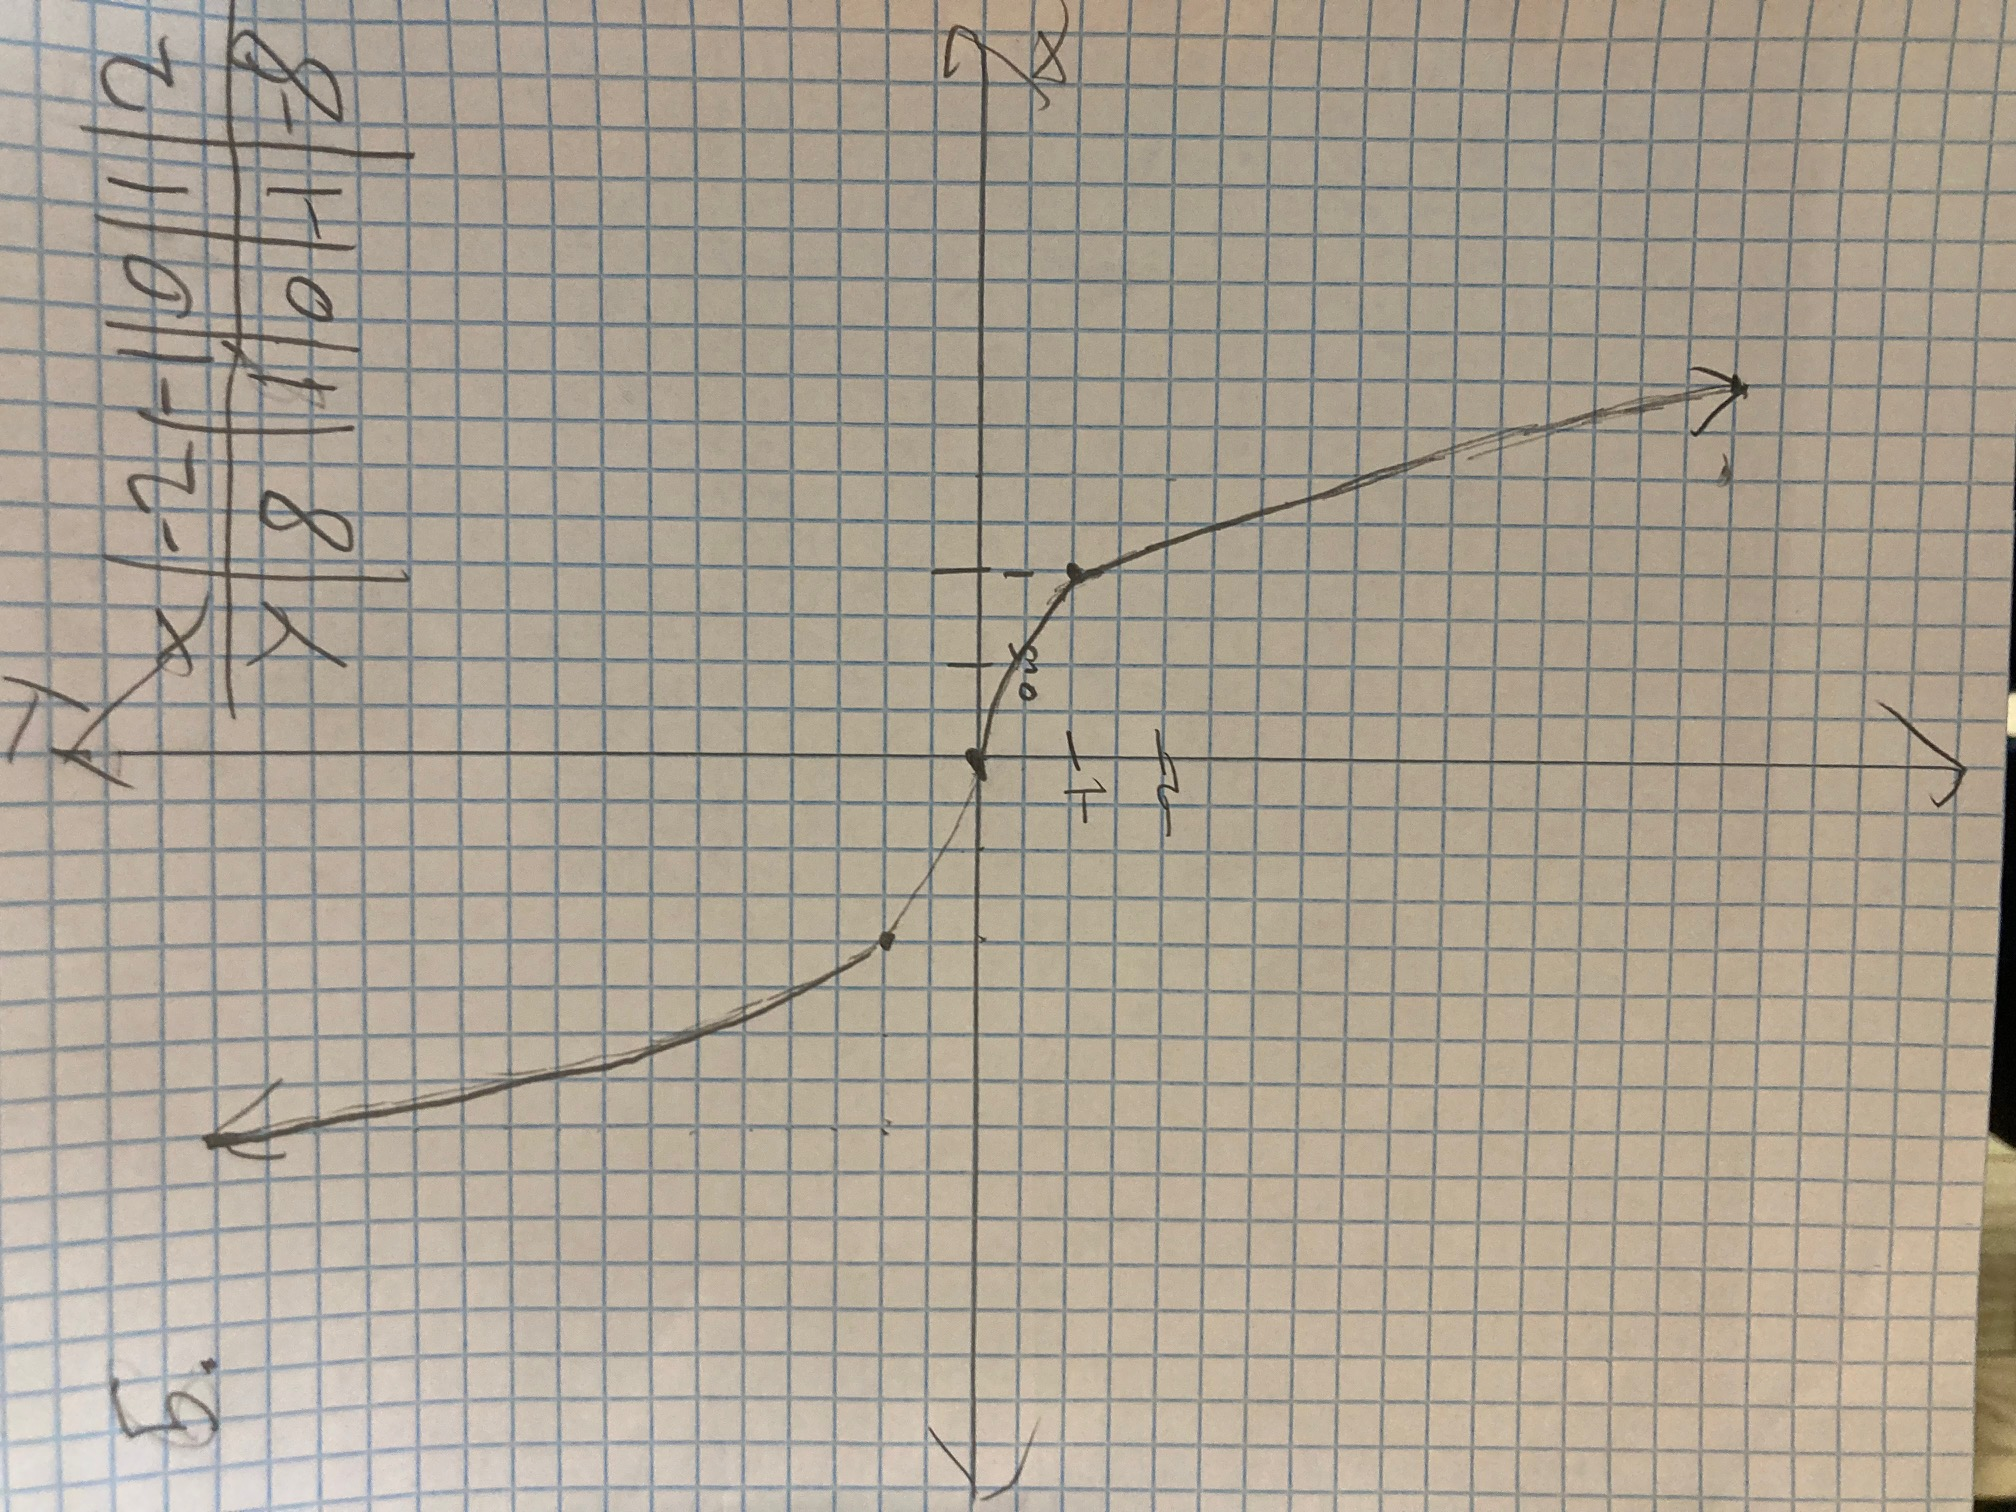
\includegraphics[width = 4in, height = 4in, angle = -90]{picture5}

\section*{6}
Because this is a polynomial of even degree (4) such that the leading coefficient is positive, $f(x)\rightarrow +\infty$ as $x\rightarrow \pm\infty$. 
Using the rational roots theorem, we can tell that this function has no rational zeros:
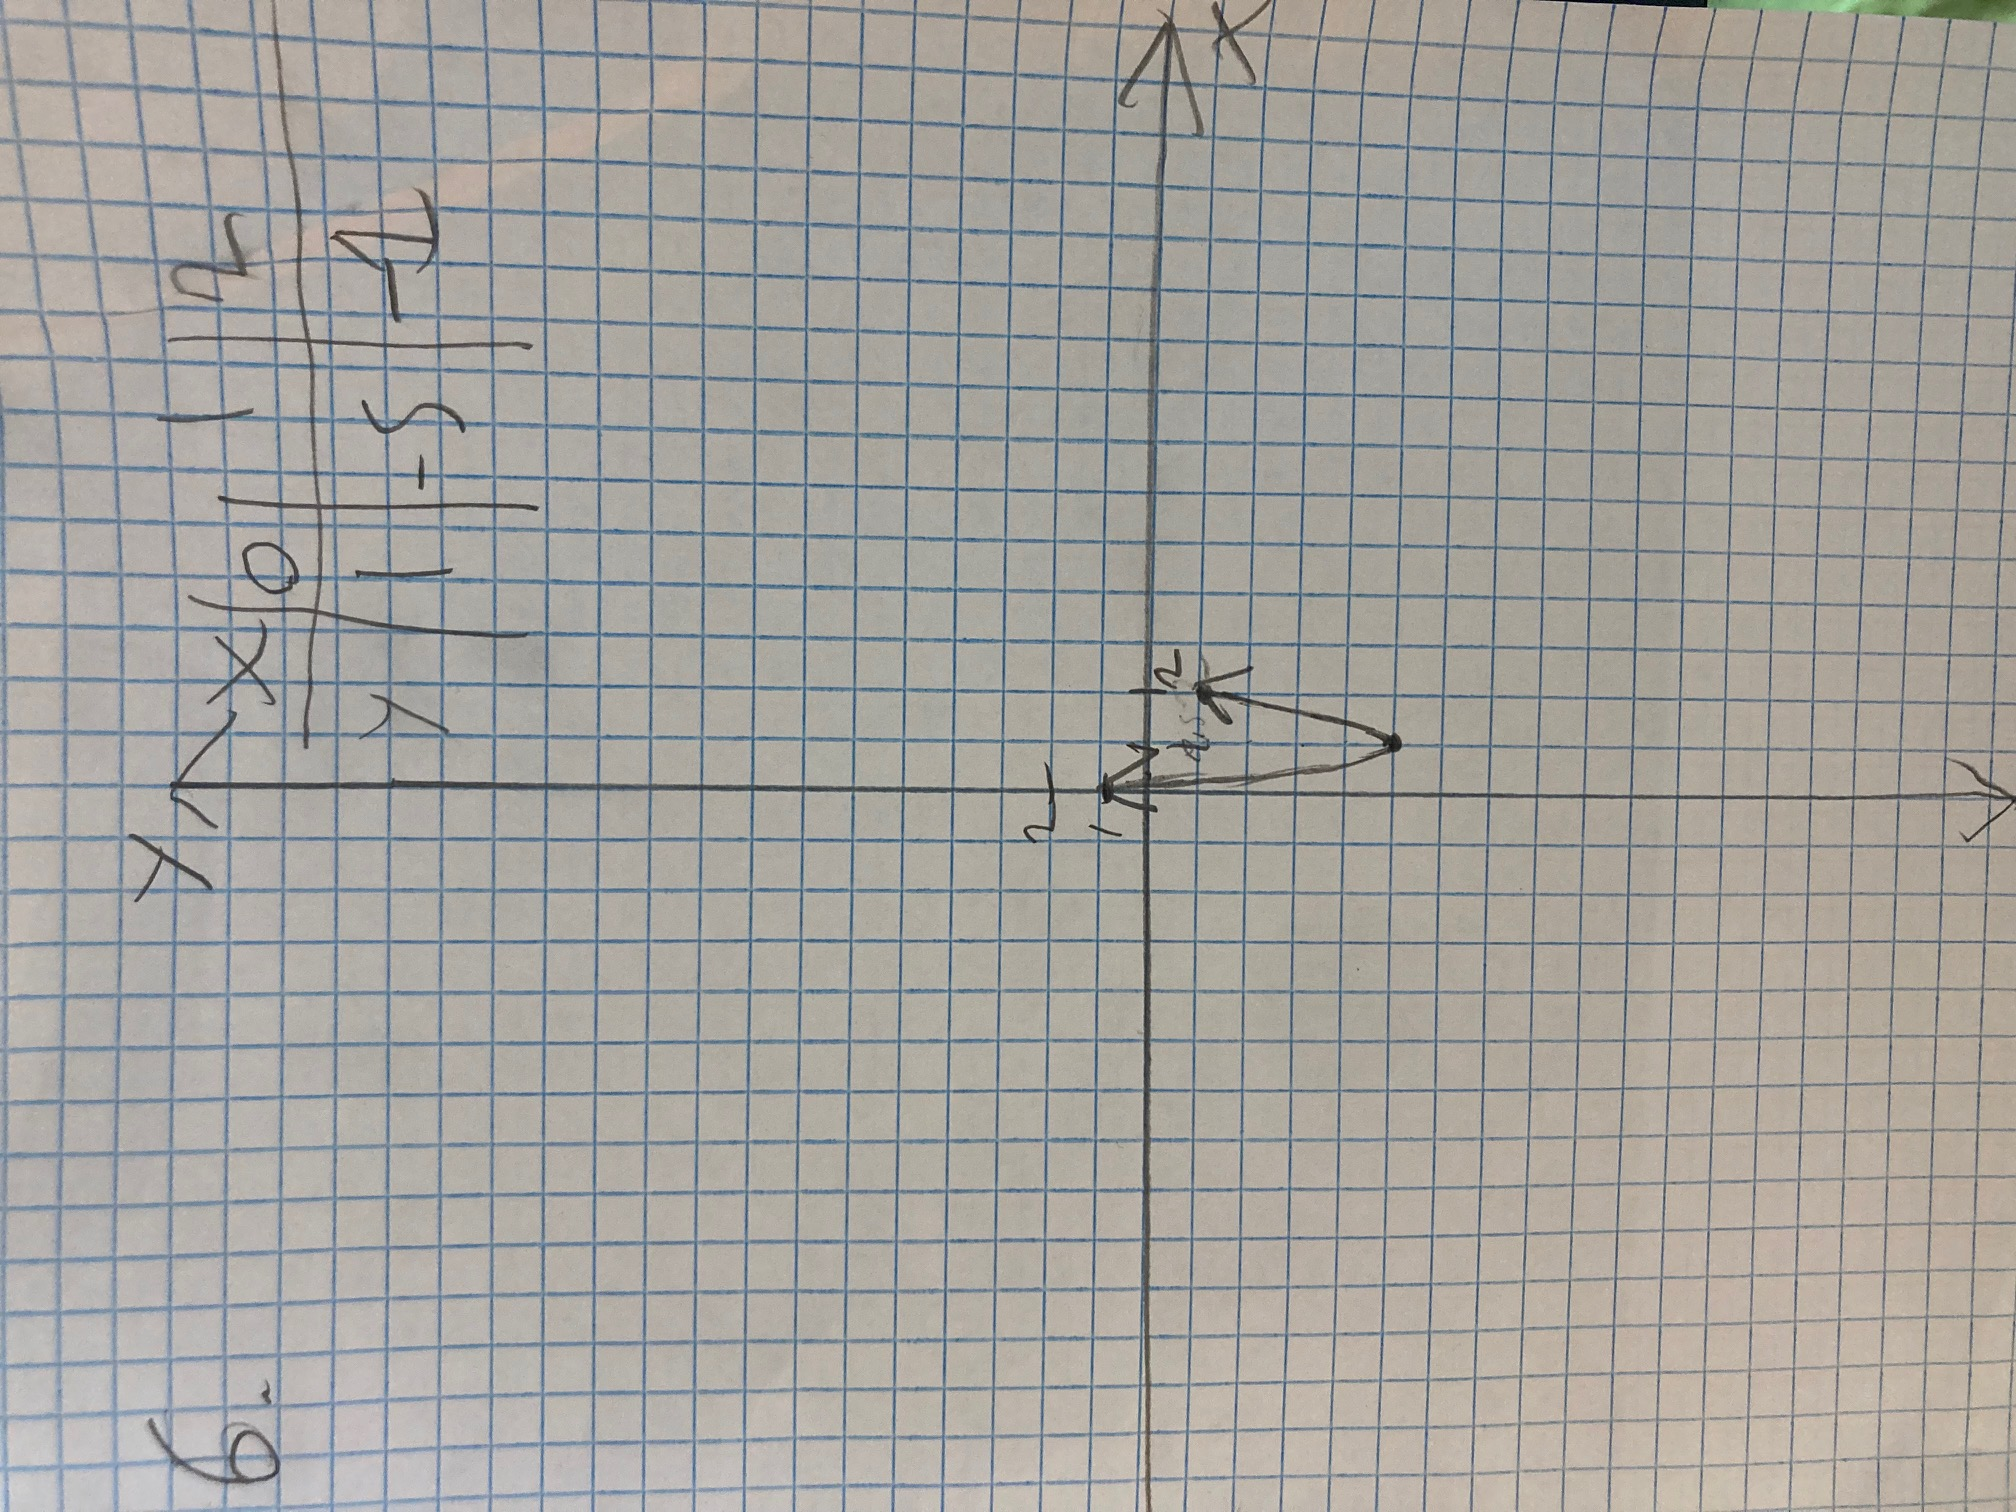
\includegraphics[width = 4in, height = 4in, angle = -90]{picture6}

\section*{7}
Because this is a polynomial of odd degree (5) such that the leading coefficient is positve, $f(x)\rightarrow +\infty$ as $x\rightarrow +\infty$, 
and $f(x)\rightarrow -\infty$ as $x\rightarrow -\infty$. By the rational roots theorem, we can tell that this polynomial has no rational zeros:
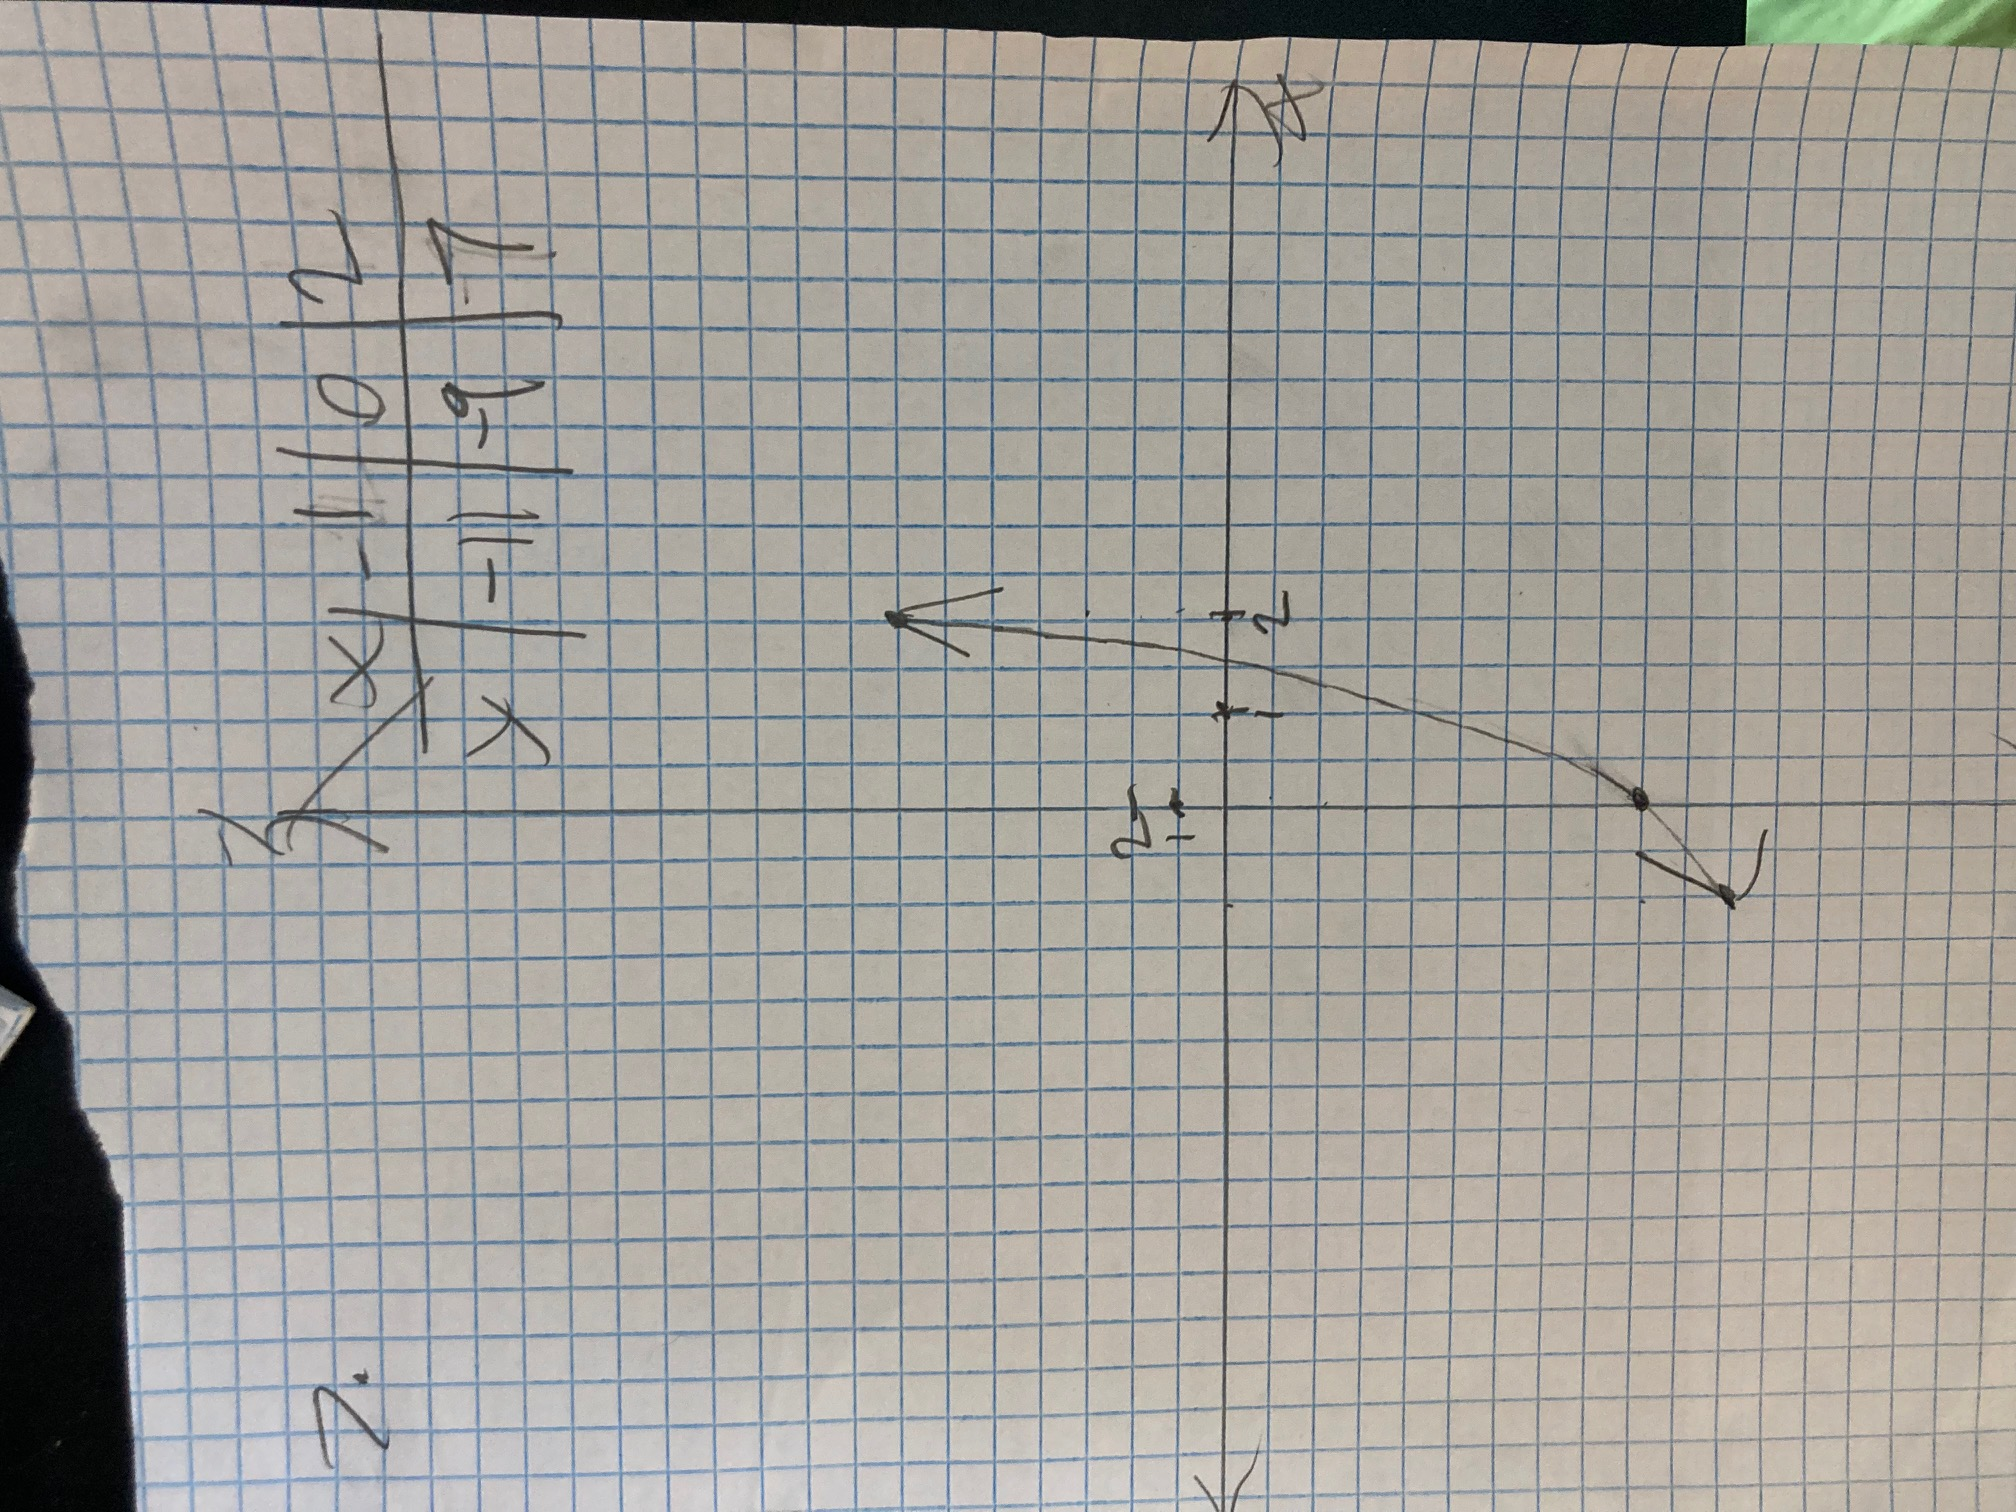
\includegraphics[width = 4in, height = 4in, angle = -90]{picture7}

\section*{8}
\[ (2x^3+5x^2-7x+4)+(x^3-3x^2-4x)=3x^3+2x^2-11x+4 \]

\section*{9}
\[ (3x^3-4x^2+3x-5)-(x^2+4x-8)=3x^3-5x^2-x+3 \]

\section*{10}
\[ (3x-2)(x^2+4x-7)=3x(x^2+4x-7)-2(x^2+4x-7)=(3x^3+12x^2-21x)-(2x^2+8x-14)=3x^3-10x^2-29x+14 \]

\section*{11}
\[ (3x-5)^3=(3x)^3-3(3x)^2(-5)+3(3x)(-5)^2-(-5)^3=27x^3+135x^2+225x+125 \]

\section*{12}
Because we are dividing by a termn $x-k$, we can use synthetic division:
\begin{center}
\begin{tabular}{r|rrrr}
	$4$ & $3$ & $-14$ & $16$ & $-22$ \\
	& & $12$ & $-8$ & $32$ \\
	\cmidrule{2-5}
	& $3$ & $-2$ & $8$ & $10$
\end{tabular}
\end{center}
meaning \[ \dfrac{3x^3-14x^2+16x-22}{x-4}=3x^2-2x+8+\frac{10}{x-4} \] 

\section*{13}
We can use polynomial long division to solve this problem:
\begin{center} \begin{tabular}{rrrrrrrrr}
	 & 	&	&	&	&	& $2x^2$ & $+2x$ & $+3$ \\
			\cline{4-9} 
	 $3x^2$ & $-3x$ & $2$ & ) & $6x^4$ & $0x^3$ & $7x^2$ & $4x$ & $-17$ \\
	 & & & & $6x^4$ & $-6x^3$ & $4x^2$ \\
	 & & & & & $6x^3$ & $+3x^2$ & $+4x$ & $-17$ \\
	 & & & & & $6x^3$ & $-6x^2$ & $+4x$ \\
	 & & & & & & $9x^2$ & $+0x$ & $-17$ \\
	 & & & & & & $9x^2$ & $-9x$ & $+6$ \\
	 & & & & & & & $9x$ & $-23$
\end{tabular} \end{center}
meaning \[ \dfrac{6x^4+7x^2+4x-17}{3x^2-3x+2}=2x^2+2x+3+\frac{9x-23}{3x^2-3x+2} \]

\section*{14}
\[ 8x^3+27=(2x+3)((2x)^2-(2x)(3)+(3)^2)=(2x+3)(4x^2-6x+9) \]

\section*{15}
\[ x^4+5x^2-6=(x^2)^2+5(x^2)-6=(x^2+6)(x^2-1) \]

\section*{16}
\[ x^3-3x^2-4x+12=x^2(x)+x^2(-3)-4(x)-4(-3)=(x^2-4)(x-3) \]

\section*{17}
We can use the rational roots theorem to determine that the possible real zeros are:
\[ \pm 1,\pm 2,\pm 4,\pm 5, \pm 8, \pm 10, \pm 20, \pm 40 \] Using a calculator, one can see that $-2$ is one such zero, meaning $x+2$ is a factor 
of the polynomial. We can use synthetic division to find the other factor:
\begin{center}
\begin{tabular}{r|rrrr}
	$-2$ & $1$ & $1$ & $-22$ & $-40$ \\
	& & $-2$ & $2$ & $40$ \\
	\cmidrule{2-5}
	& $1$ & $-1$ & $-20$ & $0$ 
\end{tabular}
\end{center}
meaning the other factor is \[ x^2-x-20=(x-5)(x+4) \] Thus, the real zeros of the polynomial are $-2,5$ and $-4$. This matches up with the fundemental 
theorem of algebra, which states that the given polynomial of degree $3$ has exactly $3$ zeros, and we have found $3$ zeros.

\section*{18}
We can use the rational roots theorem to determine that the possible real zeros are:
\[ \pm 1, \pm 2, \pm 3, \pm 6, \pm\frac{1}{2}, \pm\frac{3}{2}, \pm\frac{1}{4}, \pm\frac{3}{4} \]
Using a calculator, one can see that $-2$ is one such solution, meaning $x+2$ is a factor of the polynomial. We can then use synthetic division to find the 
other factor:
\begin{center}
\begin{tabular}{r|rrrrr}
        $-2$ & $4$ & $-8$ & $-19$ & $23$ & $-6$ \\
        & & $-8$ & $32$ & $-26$ & $6$ \\
        \cmidrule{2-6}
        & $4$ & $-16$ & $13$ & $-3$ & $0$
\end{tabular}
\end{center} 
meaning the other factor is \[ 4x^3-16x^2+13x-3 \] We can use the rational roots theorem again, and determine that one real zero of this polynomial 
is $3$. We can again use synthetic division to find the other factor:
\begin{center}
\begin{tabular}{r|rrrr}
        $3$ & $4$ & $-16$ & $13$ & $-3$ \\
        & & $12$ & $-12$ & $3$ \\
        \cmidrule{2-5}
        & $4$ & $-4$ & $1$ & $0$
\end{tabular}
\end{center}
meaning the other factor is \[ 4x^2-4x+1=(2x)^2-4x+1^2=(2x-1)^2 \] This means that the real zeros of the original polynomial are $-2,3$ and $\frac{1}{2}$. 
Because the factor $2x-1$ is counted twice, the zero $\frac{1}{2}$ is also counted twice, meaning we have found 4 zeros. This matches up with the 
fundemental theorem of algebra, which states that this polynomial of degree $4$ has exactly $4$ zeros.

\section*{19}
\[ f(x)=(x+1)(x-3)(x-4)=(x^2-2x-3)(x-4)=(x^3-2x-3x)-(4x^2-8x-12)=x^3-6x^2+5x+12 \]

\section*{20}
By the complex conjugates theorem, we know that if $2i$ is a zero of $f$, then so is $-2i$:
\[ f(x)=(x-6)(x+2i)(x-2i) \]

\section*{21}
By the irrational conjugates theorem, we know that if $1-\sqrt{5}$ is a zero of $f$, then so is $1+\sqrt{5}$:
\[ f(x)=(x+3)(x+1)(x-(1-\sqrt{5}))(x-(1+\sqrt{5})) \]

\section*{22}
By the complex conjugates theorem, we know that if $1+3i$ is a zero of $f$, then so is $1-3i$. By the irrational conjugates theorem, we know that if 
$4+\sqrt{10}$ is a zero of $f$, then so is $4-\sqrt{10}$:
\[ f(x)=(x-(1+3i))(x-(1-3i))(x-(4+\sqrt{10}))(x-(4-\sqrt{10})) \]

\section*{23}
Because this function is of degree $3$, we know that it has at most $2$ turning points. These are $(0.333,4.481)$ and $(3,-5)$.

\section*{24}
Because this function is of degree $4$, we know that it has at most $3$ turning points. Using a calculator, we can see that it has one turning point:
$(-2.652,-27.436)$.

\section*{25}
After plotting the points, we can see that, from the graph, there are no visible turning points after sketching curves from the points. We can also 
clearly see that it is not of degree $1$ or $0$, therefore meaning that the least degree of the function is $2$, a quadratic.

\section*{26}
After sketching the graph, we can see that there are two visible turning points. Because a polynomial of degree $n$ has at most $n-1$ turning points, 
this means that the lowest degree this graph could have would be of degree $3$, a cubic.

\section*{27}
The per capita GDP can be found by dividing the GDP by the population. We know that the GDP was about $1.099\times 10^{13}$ dollars, while the 
population was about $2.91\times 10^8$, meaning the per capita GDP was:
\[ \frac{1.099\times 10^{13}}{2.91\times 10^8}=0.378\times 10^5=3.78\times 10^4 \] dollars.

\section*{28}
The error here is that the possible rational zeros listed are those of the form $\frac{q}{p}$ where $q$ is the leading coefficient and $p$ is 
the constant term. Instead, the rational roots theorem states that those possible rational zeros are of the form $\frac{p}{q}$. Thus, the possible 
rational zeros are:
\[ \pm 1, \pm 2, \pm 4, \pm 8, \pm 16, \pm\frac{1}{2}, \pm\frac{1}{4},\pm\frac{1}{8} \]

\section*{29}
We know that the volume of a rectangular prism is given by \[ V=lwh \] We can substitute in the given values to find the value of $x$:
\[ 1040=x(x+2)(2x-3)=(x^2+2x)(2x-3)=(2x^3-3x^2)+(4x^2-6x)=2x^3+x^2-6x \]
\[ 2x^3+x^2-6x-1040=0 \]
Using the rational roots theorem, we can determine that one real zero of this function is $8$, meaning $x-8$ is a factor of the polynomial. Using 
synthetic division, we can find the other factor:
\begin{center}
\begin{tabular}{r|rrrr}
	$8$ & $2$ & $1$ & $-6$ & $-1040$ \\
	& & $16$ & $136$ & $1040$ \\
	\cmidrule{2-5}
	& $2$ & $17$ & $130$ & $0$
\end{tabular}
\end{center}
meaning the other factor is \[ 2x^2+17x+130 \] For this quadratic, because $b^2-4ac=17^2-4(2)(130)=-751<0$ we know that it has no real zeros. Thus, 
the only real zero of the initial equation for the volume is $8$, meaning $x=8$, and therefore, the dimensions of the rectangular prism are 
$8,8+2=10$ and $2(8)-3=13$ inches.
\end{document}
